\vspace{-3mm}
\section{Ablation Study: \kern -0.3em \envname \kern -0.1em is Robust}

We conduct ablation studies on both hyperparameters and model selection. The results show that \envname consistently produces high-quality simulations across a range of settings, demonstrating strong robustness. Detailed experimental configurations are provided in Appendix~\S\ref{ablation-study-details}.



\begin{figure*}[t]
    \centering
    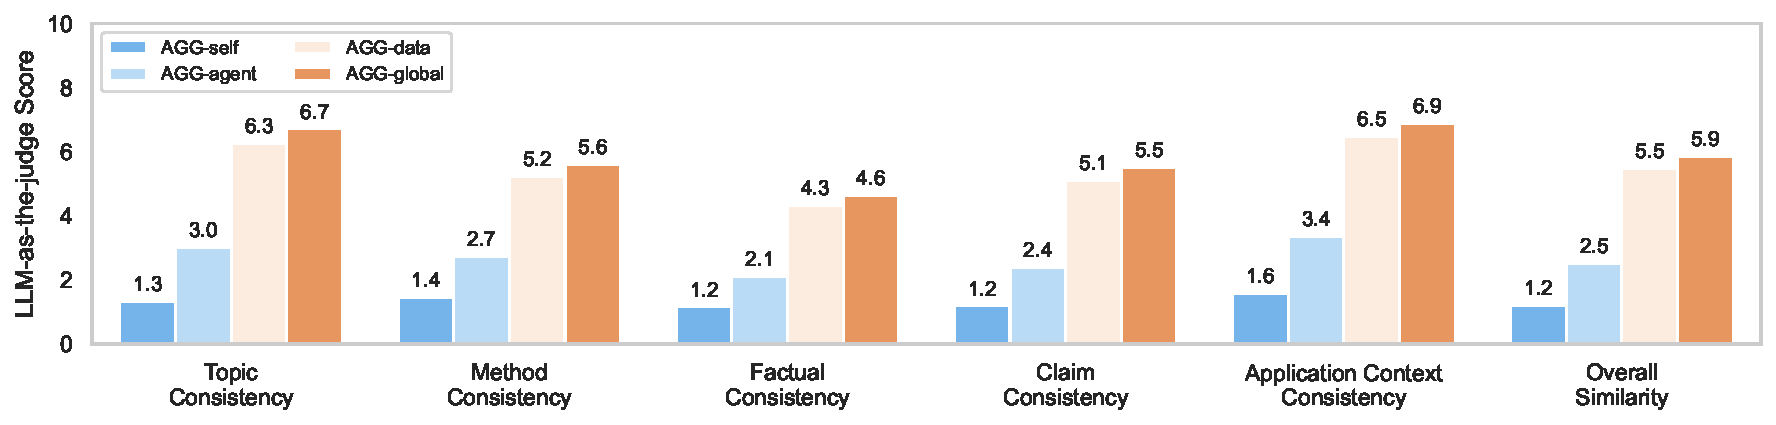
\includegraphics[width=\linewidth]{figs/llm_prompting.pdf}
    \par\vspace{-3.5mm}
    \caption{\textbf{Fine-grained similarity evaluation using LLM-as-a-judge for paper writing simulation.} We use GPT-4o as the evaluator, prompting it to score each dimension on a scale from 0 to 10. The first five dimensions assess specific aspects of similarity, while the final score (\textit{overall similarity}) represents an overall score as judged by the LLM.}
    \label{fig:fine-grained-similarity}
    \vspace{-3mm}
\end{figure*}

\xhdr{Ablation on paper number}
In paper writing tasks, users can freely assign papers to simulate non-existent work, making robustness to the number of papers essential. As shown in Figure~\ref{paper_writing_paper_number}, papers cited in the related work section have the greatest positive impact, increasing the similarity score from 66.4 to 66.7 compared to using all papers. In contrast, using only papers cited in the introduction lowers the score to 65.2, while including papers from other sections reduces it further to 58.4. These results highlight the importance of selecting informative references when generating papers. In review writing, the number of papers is fixed, so no ablation study on the paper number is applicable.

\xhdr{Ablation on agent number}
For \envname simulation, users can assign different numbers of agents, making robustness to agent number critical for \envname. In Figure~\ref{paper_writing_researcher_num}, in the paper writing task, increasing the agent number improves simulation quality under the agent-aggregation setting. The most notable gain occurs when increasing from 1 to 2, boosting the similarity score from 49.0 to 52.7.
Similar trends hold in review writing (Figure~\ref{review_writing_researcher_num}), where increasing the agent number consistently enhances output quality. The strength score improves from 50.8 to 51.5 when increasing the reviewer from 1 to 5.



\xhdr{Ablation on generation models} The choice of LLMs significantly impacts simulation quality. In addition to GPT-4o-mini, we evaluate two models from different families: Qwen-2.5-7B-Instruct\footnote{\url{https://huggingface.co/Qwen/Qwen2.5-7B-Instruct}} and Deepseek-v3\footnote{We point \texttt{DeepSeek-V3-0324} for use.}. In Table~\ref{tab:model-ablation}, for both paper writing tasks, global aggregation (\envname) consistently yields the highest similarity scores across all models. It also achieves the best review difference scores for Qwen-2.5-7B-Instruct and Deepseek-v3. The only exception is GPT-4o-mini, which shows an unexpected increase in review difference under AGG-global. Overall, Deepseek-v3 outperforms GPT-4o-mini, which in turn outperforms Qwen-2.5-7B-Instruct—consistent with their relative performance on other tasks.

\xhdr{Ablation on embedding models} Similarity scores can be computed using different models, and voyage-3\footnote{\url{https://blog.voyageai.com/2024/09/18/voyage-3/}} serves as an alternative to the text-embedding-3-large used in our main experiments. As shown in Figures~\ref{paper_writing_paper_number}, \ref{paper_writing_researcher_num}, and \ref{review_writing_researcher_num}, voyage-3 produces consistent trends in ablation studies involving the number of papers and agents. This consistency suggests that \envname is robust to the choice of embedding model, and different models lead to the same conclusions.



\vspace{-1mm}
\section{Discussion: \envname is Effective}
Besides computing embedding-based similarities, we provide more types of evaluations here. First, we prompt LLMs to calculate fine-grained similarity scores that assess consistency between real-world data and simulated ones across various dimensions. Next, we evaluate the intrinsic quality of the simulated outputs themselves and compare them with real-world data. Finally, we report results from human evaluations to validate the alignment between LLM-based evaluation and human judgments. More details about LLM-based evaluation are available in Appendix~\S\ref{sec:llm-based-eval}, and details about human evaluation are available in Appendix~\S\ref{sec:human-eval}.

\xhdr{Automatic evaluation on fine-grained similarity} A high cosine similarity score alone can mask important issues in simulated results.
To capture a more complete picture of similarity, we move beyond a single score and instead evaluate across five fine-grained dimensions: \textit{topic consistency}, \textit{method consistency}, \textit{factual consistency}, \textit{claim consistency}, and \textit{application context consistency}. These dimensions collectively reflect subcomponents of overall semantic similarity. For evaluation, we use GPT-4o to assign scores from 0 to 10 for each dimension for each paper. As shown in Figure~\ref{fig:fine-grained-similarity}, our proposed global aggregation method (\envname) consistently outperforms all other aggregation baselines across these dimensions. This demonstrates that \envname provides a more effective simulation of research activities compared to baselines. 


\begin{table}[t]
\setlength\tabcolsep{5pt}
\centering
\small
\caption{\textbf{Comparison of simulation results with different generation models.} For \textit{Qwen}, we refer to Qwen-2.5-7B-Instruct. For \textit{GPT}, we refer to GPT-4o-mini. For \textit{DS}, we refer to Deepseek-v3. For paper writing metrics, we utilize the overall similarity. For review writing metrics, we use $\Delta\mb{S}$ to represent its review alignment with the real world.}
\begin{tabular}{lcccccc}
\toprule
\multirow{2}{*}{\textbf{AGG Type}} & \multicolumn{3}{c}{\textbf{Paper Writing}} & \multicolumn{3}{c}{\textbf{Review Writing}} \\
\cmidrule(lr){2-4} \cmidrule(lr){5-7}
 & Qwen & GPT & DS & Qwen & GPT & DS \\
\midrule
AGG-self       & 46.45 & 46.08 & \underline{48.62} & 1.36 & 1.27 & \underline{1.11} \\
AGG-agent      & 53.91 & 55.24 & \underline{56.19} & 1.41 & 1.19 & \underline{1.05} \\
AGG-data       & 65.03 & \underline{65.30} & 65.05 & 1.28 & 1.26 & \underline{1.07} \\
AGG-global     & 65.30 & \underline{67.51} & 65.33 & \underline{0.79} & 1.51 & 0.81 \\
\bottomrule
\end{tabular}
\vspace{-4mm}
\label{tab:model-ablation}
\end{table}



\begin{table}[t]
\setlength\tabcolsep{4pt}
\centering
\small
\caption{\textbf{Evaluation results on novelty and feasibility.} Each paper is assigned scores from 0 to 10 for novelty and feasibility. Both LLM-based evaluation and human evaluations are conducted to evaluate the quality of simulated papers. LLM-based evaluation includes results on 1,000 papers, and human evaluation includes results on 40 of them. \textit{Simulation} represents the outputs of \envname, \textit{real-world} represents the existing papers.}
\begin{tabular}{lcccc}
\toprule
\multirow{2}{*}{\textbf{Evaluation}} & \multicolumn{2}{c}{\textbf{Simulation}} & \multicolumn{2}{c}{\textbf{Real-world}} \\
\cmidrule(lr){2-3} \cmidrule(lr){4-5}
 & \textbf{Novelty} & \textbf{Feasibility} & \textbf{Novelty} & \textbf{Feasibility} \\
\midrule
LLM-based & 7.39 & 6.82 & \underline{7.85} & \underline{7.13} \\
Human-based &  5.50 & \underline{7.98} & \underline{5.90} & 7.85 \\
\bottomrule
\end{tabular}
\vspace{-5mm}
\label{tab:novelty_feasibility}
\end{table}


\begin{figure*}[t]
    \centering
    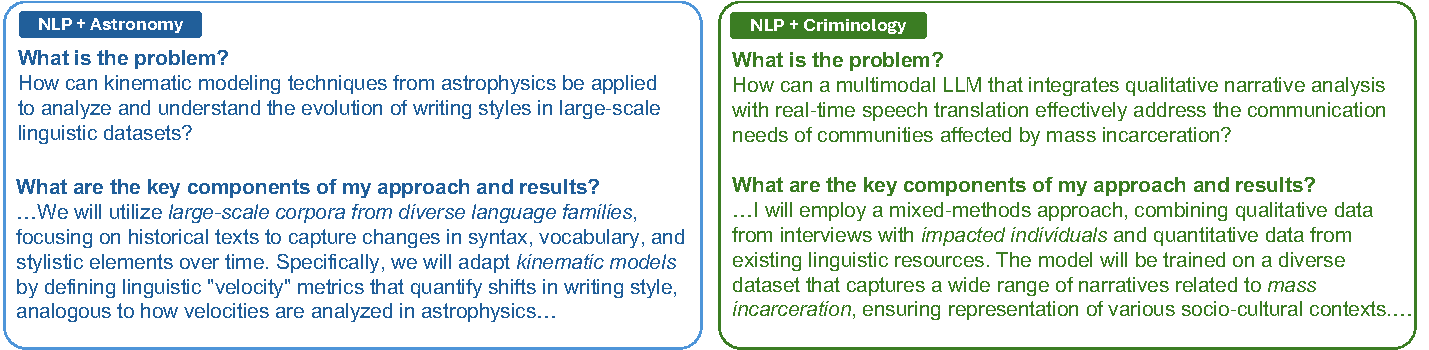
\includegraphics[width=\linewidth]{figs/case_study.pdf}
    \caption{\textbf{Examples of generated interdisciplinary research papers from \envname}. For each example, we include \envname's responses to two questions: ``\textit{What is the problem?}'' and ``\textit{What are the key components of my approach and results?}'' as these are the most critical among the five questions mentioned in Appendix~\S\ref{evaluation-details}. Appendix~\S\ref{additional-case-study} provides the full contents of the above two and more examples for interdisciplinary research.}
    \label{fig:case-study}
    \vspace{-4mm}
\end{figure*}


\xhdr{Automatic evaluation on intrinsic quality} In addition to evaluating semantic similarity between simulated and real-world data, we also assess the intrinsic quality of the generated content. Specifically, we focus on two key dimensions: \textit{novelty} and \textit{feasibility}, which we consider the two most critical aspects of a research proposal. As shown in Table~\ref{tab:novelty_feasibility}, the simulated outputs still do not match the novelty and feasibility levels of real-world articles but are close to those. This gap indicates that \envname would benefit from a more coordinated agentic workflow to enhance the quality of the generated research outputs.

\xhdr{Human evaluation} Evaluation based on LLMs may introduce bias into the results. To validate the reliability of LLM-based evaluations, we conduct additional human evaluations. For similarity-based assessments, human judgments correlate well with LLM scores, achieving a Pearson correlation of 0.61, indicating reasonable agreement. However, for intrinsic quality evaluations, the correlation between human and LLM scores is low. This is likely due to the inherent ambiguity of such tasks and the need for domain-specific expertise. Despite this, both human and LLM evaluations consistently indicate that simulated papers are slightly less novel than real-world ones—though the gap is relatively small (5.50 vs 5.90 for humans and 7.39 vs 7.85 for LLMs).



